\begin{tikzpicture}[transform canvas={scale=0.9}] 
  \begin{scope}[yshift=0.2\textwidth]
    \begin{scope}[xshift=0cm]
      \node [mybox] (all) at (0, 0) {
	  \begin{tabular}{c}
	  {\small $( \SE + \RQ ) \times ( \Per + \CS)$  } \\	  
        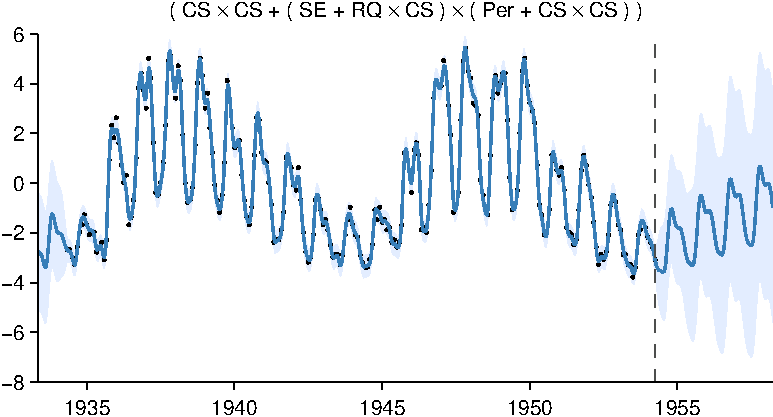
\includegraphics[trim=0 0 0 1.2cm, clip, width=0.8\textwidth, height=0.28\textwidth]{figures/radio/all.pdf}
		\end{tabular}
      };
    \end{scope}
  \end{scope}
  \begin{scope}[yshift=0.3\textwidth]
    \begin{scope}[xshift=4.8cm]
        \node [mybox, below of=all] (equals) at (0, 0) {\Huge{$=$}};
    \end{scope}
  \end{scope}
  \begin{scope}[yshift=-0.11\textwidth]
    \begin{scope}[xshift=-0.3\textwidth]
      \node [mybox] (all) at (0, 0) {
	  	  \begin{tabular}{c}
	  {\small $\SE$ } \\	 
        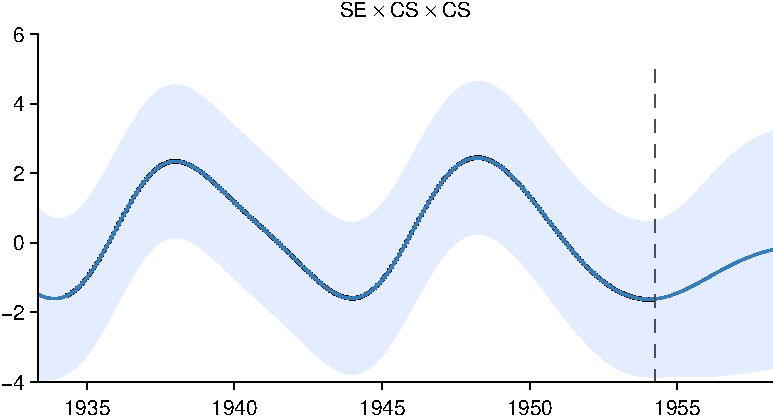
\includegraphics[trim=0 0 0 1.1cm, clip, width=0.5\textwidth, height=2.2cm]{figures/radio/3.pdf}
		\end{tabular}
      };
    \end{scope}
    \begin{scope}[xshift=+0.3\textwidth]
      \node [mybox] (all) at (0, 0) {
	  	  \begin{tabular}{c}
	   {\small $\Per \times \RQ$ } \\	 
        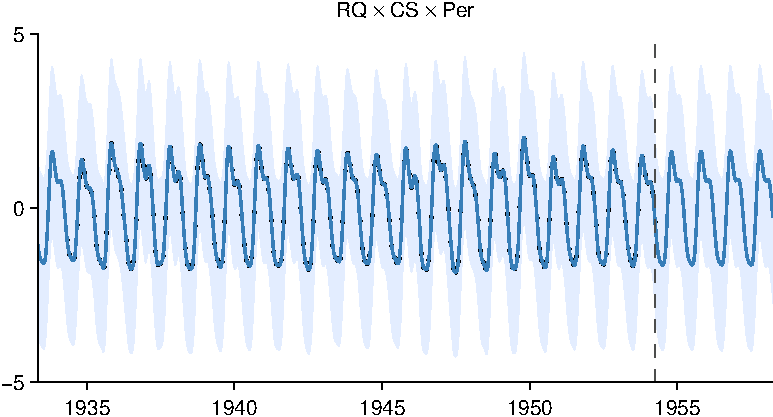
\includegraphics[trim=0 0 0 1.1cm, clip, width=0.5\textwidth, height=2.2cm]{figures/radio/4.pdf}
		\end{tabular}
      };
    \end{scope}
  \end{scope}
  \begin{scope}[yshift=-0.16\textwidth]
    \begin{scope}[xshift=0cm]
        \node [mybox, below of=all] (equals) at (0, 0) {\Huge{+}};
    \end{scope}
  \end{scope}
  \begin{scope}[yshift=-0.38\textwidth]
    \begin{scope}[xshift=-0.3\textwidth]
      \node [mybox] (all) at (0, 0) {
	  	  \begin{tabular}{c}
	  {\small $\Per \times \SE$ } \\	 
        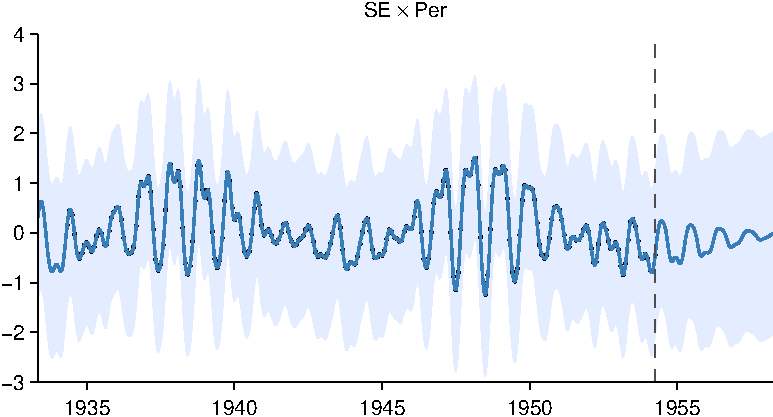
\includegraphics[trim=0 0 0 1.1cm, clip, width=0.5\textwidth, height=2.2cm]{figures/radio/2.pdf}
		\end{tabular}
      };
    \end{scope}
    \begin{scope}[xshift=+0.3\textwidth]
      \node [mybox] (all) at (0, 0) {
	  	  \begin{tabular}{c}
	  {\small $\RQ$ } \\	 
        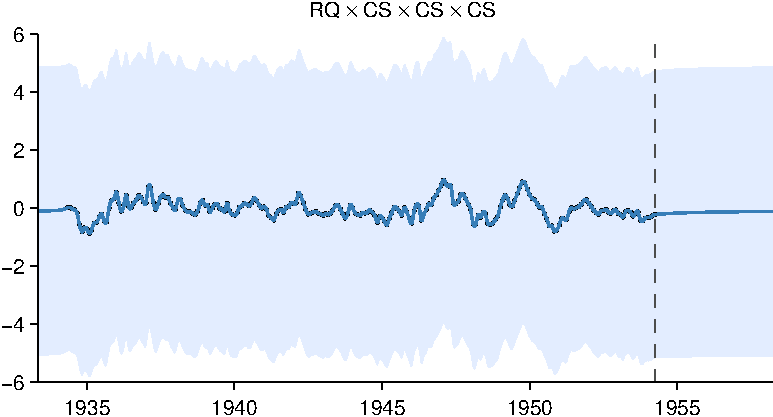
\includegraphics[trim=0 0 0 1.1cm, clip, width=0.5\textwidth, height=2.2cm]{figures/radio/5.pdf}
		\end{tabular}
      };
    \end{scope}
  \end{scope}
\end{tikzpicture}
